% !TeX root = ../main.tex
% Add the above to each chapter to make compiling the PDF easier in some editors.

\chapter{Methodology}\label{chapter:methodology}

\section{Selection Criteria}
The core aim of this research study involves examining and evaluating
various publicly available deepfake detection tools. It becomes imperative
to establish a well-defined set of selection criteria for these tools.
Selecting the right criteria is essential not just for representing a variety
of detection methods, but also for making a fair comparison between the tools.
The objective is to ensure that the evaluated tools are understandable,
encompassing the nuances of accessibility, ease of use, limitations, variety
in detection methods, and documentation. These are the criteria used to select the tools:

\textbf{Ease of Use and Limitations.} The tools were chosen based on their ease of
operation. Considerations included the installation process of the chosen tool,
the availability of \ac{API}, and whether a user with IT skills could utilize
these APIs for integration purposes. Questions were raised about the specific
operating systems needed, the requirement of a constant internet connection,
and any inherent limitations of the tools. Do the developer or owner of the
tool make any specific promises or claims about its use? Additionally, do the
tools have restrictions on file soze or video length, and do these factors
matter to use the tools?

\textbf{Accessibility.} Questions about the tools' accessibility include their
public availability, any special account requirements for access, and if they can
run on standard PCs or laptops. Can the tools be accessed via a website or is specialized
software platforms like GitHub, Hugging Face or Google Colab or an \ac{IDE} required?
The need for enhanced \ac{GPU} or other hardware specifications, as well as the nature
of the tool (open source vs.\ proprietary), were also considered.

\textbf{Support and Documentation.} Factors taken into account included the
provision of user support, installation guidance, usage documentation, and
resources for development. The existence of troubleshooting resources,
community discussions for Q\&A, and availability of the source code for
developers' adaptability were important considerations.

\textbf{Difficulty of Use.} The complexity of the tools was evaluated on different levels.
It was labeled as \textit{Easy} if the tool was web-based with a user-friendly
interface for detecting deepfakes and if there is any \ac{API}s available. \textit{Moderate} 
if it provided a platform like Hugging Face Space or Google Colab, and \textit{Challenging} 
if users had to devise their own way to utilize the tool.

\textbf{Cost Considerations.} Determined whether the tool is free or comes with a
subscription fee, emphasizing a preference for freely available options. Also, if
paid versions existed, did they provide additional functionality or ease of use?

\textbf{Privacy Policy.} The presence of privacy policies and terms of use for the
tools was verified, underscoring their importance for tool legitimacy and
trustworthiness. Especially when users are required to log in, it's essential
to clarify how personal information is managed. Additionally, statements regarding
ethical issues and adherence to relevant laws and regulations further bolster the
tool's credibility and users' confidence in its operations.

The aforementioned criteria that were established played a critical role in the
selection process of the tools. Tools were preferred that could be easily
accessed and trusted by a broad audience. By ensuring tools had clear easy
installations and user-friendly interfaces, the safety and simplicity of the
selected tools were prioritized. It wasn't just about identifying 
publicly-available tools; the goal was to ensure the chosen tools covered not just
accessibility needs, but were also user-friendly enough for individuals without
deepfake expertise. This approach aimed to make the tools both dependable and
user-friendly, addressing a variety of user requirements.

An overview of the selection criteria is provided in~\autoref{tab:selection_criteria}.

\begin{table}[htpb]
	\caption{Selection Criteria}\label{tab:selection_criteria}
	\centering
	\small
	\begin{tabularx}{\textwidth}{l X}
		\toprule
		\textbf{Selection Criteria} & \textbf{Description}                                      \\
		\midrule
		Ease of Use and Limitations & The tool's user-friendliness is determined
		by the simplicity of its installation process and operational
		requirements. Is it a straightforward drag-and-drop mechanism, or does
		it demand any special software? Additionally, any constraints, such
		as file size limits or video duration caps, play a role in its overall
		user-friendliness.                                                                      \\
		\addlinespace
		Accessibility               & Only publicly-available tools were considered
		to ensure broad user accessibility. The ease of use, from browser access
		to local installation, and hardware demands, with a preference for
		standard configurations or cloud solutions like Google Colab,
		were pivotal in evaluations.                                                            \\
		\addlinespace
		Support and Documentation   & Proper documentation and active support,
		be it community or developer-driven, are crucial. Regular support
		ensures that users can fully make use of tool features, troubleshoot issues,
		and gain deeper insights into the tool's functionalities.                               \\
		\addlinespace
		Difficulty of Use           & The tool's complexity was categorized as
		\textit{Easy} for web-based interfaces and with \ac{API} offer, \textit{Moderate} for those using
		platforms like Hugging Face or Google Colab, and \textit{Challenging}
		when users needed a custom approach.                                                    \\
		\addlinespace
		Cost considerations         & It is assessed if the tool is free or
		subscription-based, favoring free options, and checked if paid versions
		offered enhanced features or usability.                                                 \\
		\addlinespace
		Privacy Policy              & Tools were evaluated for privacy policies and user terms,
		emphasizing trust. It's vital to know how tools handle login data and their
		stance on ethics and legal compliance to ensure credibility.                            \\
		\bottomrule
	\end{tabularx}
\end{table}

\section{Evaluation Metrics}
After careful selection of the tools based on the prescribed criteria, it is
important to systematically evaluate them to ensure their, accuracy
and efficiency. This evaluation isn't just about how these tools perform; it's
about understanding their strengths and potential weaknesses.

Each tool has a unique set of features and algorithms that drive its functionality.
However, to compare them on a fair level and to ensure a comprehensive
assessment, a standard set of evaluation metrics is applied. These are the evaluation
metrics that were selected:

\textbf{Processing Time and Scalability.} The time taken for an input to be analyzed
and authenticated by the tool is important. An average processing time, represented
by average seconds, was used in this assessment. The tool's ability to process multiple
images or videos simultaneously and subsequently produce an output list indicating
the authenticity of each piece of content was also examined.

\textbf{Interpretability.} The quality of the output produced by a tool was assessed
based on its clarity and simplicity. Inputs were checked if they were simply labeled
as `Real' or `Fake', or if a probabilistic estimate indicating the likelihood of
manipulation was provided. When probabilities were presented, the format
(whether in percentages) and the threshold at which content was termed as a deepfake
were investigated. In this study, content was classified as a deepfake if a
probability of 50\% or higher was observed.

\textbf{Detection Accuracy.} The fraction of true outcomes (including both true
positives and true negatives) within the entire dataset was analyzed. This served
to understand the tool's aptitude in correctly differentiating genuine from manipulated
content.

\textbf{Precision.} The fraction of true positive outcomes within the total predicted
positives (including both true and false positives) was evaluated. The tool's capacity
to minimize false positives, ensuring that genuine content wasn't incorrectly flagged,
was assessed.

\textbf{Recall.} The efficiency of the tool in correctly identifying actual deepfakes
from all the presented deepfakes was evaluated. The actual true positives that were
successfully identified by the tool were calculated.

\textbf{F1-Score.} The F1-Score is the harmonic mean of precision and recall, providing
a single metric that balances the trade-off between correctly identifying positive
instances (precision) and the ability to detect all potential positive instances (recall),
especially useful in situations where the class distributions are imbalanced\footnote{The class
	imbalance problem typically occurs when there are many more instances of some
	classes than others~\cite{JAVAHERI2014153}.}.

\textbf{Dataset Compatibility.} The adaptability of a tool, based on the datasets it
could align with, was explored. Tools that could function with a variety of datasets
or those that came recommended with particular datasets were chosen.

\textbf{Training Models.} The types and quality of training models and techniques that
were employed by each tool were explored.

\textbf{Programming Language and Framework.} The programming languages and frameworks
that were important in the tool's development were reviewed to gain insights into its
structure and potential functionalities.

\textbf{Potential for Further Development.} The possibility of whether tools could
undergo extended development was investigated. Furthermore, the guidelines or
requirements provided for such advancements, if any, were examined.

\begin{table}[htpb]
	\caption{Evaluation Metrics}\label{tab:evaluation_metrics}
	\centering
	\small
	\begin{tabularx}{\textwidth}{l X}
		\toprule
		\textbf{Evaluation Metrics}         & \textbf{Description}                              \\
		\midrule
		Processing time and Scalability     & Evaluates the tool's speed in detecting deepfakes
		and its performance with larger or multiple inputs.                                     \\
		\addlinespace
		Interpretability                    & Evaluates the clarity and transparency of the
		tool's output, ensuring users can understand the detection results.                     \\
		\addlinespace
		Detection Accuracy                  & Measures the correct identification of both
		genuine and deepfake content in the dataset, encompassing true positives and true
		negatives.                                                                              \\
		\addlinespace
		Precision                           & Measures the tool's capacity to avoid false
		positives by calculating the proportion of true positive results in the total
		predicted positives, including both true and false positives.                           \\
		\addlinespace
		Recall                              & Measures the tool's accuracy in identifying
		actual deepfakes among all presented genuine content by calculating the number
		of true positives, it identifies.                                                        \\
		\addlinespace
		F1-Score                            & The harmonic mean of Precision and Recall.
		It provides a balance between the two when there's an uneven class distribution.        \\
		\addlinespace
		Dataset Compatibility               & The tool's adaptability was checked by its
		dataset compatibility. Versatile tools or those recommended for specific datasets
		were preferred.                                                                         \\
		\addlinespace
		Training Models                     & The training models and techniques used by
		each tool were examined.                                                                \\                                             \\
		\addlinespace
		Programming Language and Framework  & The programming languages and frameworks used
		in the tool's development were analyzed for insights into its capabilities.             \\
		\addlinespace
		Potential for Further Development & The potential for tool enhancement was assessed,
		along with any provided guidelines for such improvements.                               \\
		\bottomrule
	\end{tabularx}
\end{table}

These metrics serve as a guiding light, distinguishing the capabilities of each tool
in terms of detecting deepfakes. For example, the F1-Score shows how well a tool can
find fake content while avoiding mistakes. These metrics give a clear picture of a
tool's quality. Unlike selection criteria, evaluation metrics focus on how well the
tool works. By using these metrics, we can see which tools perform best and
where they might have problems. This makes it easier for researchers and users to
choose the right tool for their needs.
An overview of the evaluation metrics used in this study is provided in~\autoref{tab:evaluation_metrics}.

\section{Datasets}
Datasets are very important when working with deepfakes. They form the backbone of both
the creation and detection of deepfakes. They also help us train models to create or spot
deepfakes. Today, there are many datasets available that focus on both deepfake images
and videos~\cite{deepfake-dataset,zi2020wilddeepfake,10.1145/3531536.3532946}.
In~\autoref{fig:sample-deepfakes} a fake sample image of each dataset is provided.

\subsection{FaceForensics++}\label{section:ff++}
\ac{FF++}~\footnote{\url{https://github.com/ondyari/FaceForensics}} serves as a
broad dataset designed for forensic studies. It
comprises 977 videos sourced from YouTube, over 1,000 unique sequences, and an
impressive collection of more than 8,000 Deepfake videos~\cite{roessler2019faceforensicspp,masters-thesis}.
Originally launched in 2018, the dataset received significant updates in 2019~\cite{masters-thesis},
making it richer and more diverse. As highlighted by the creators in their 2019 paper~\cite{roessler2019faceforensicspp},
the videos in the dataset were modified using a mix of techniques. This includes two
graphics-driven methods, namely Face2Face~\cite{thies2020face2face} and FaceSwap~\cite{faceswap},
as well as two methods used in machine learning: DeepFakes~\cite{faceswap-deepfake}
and Neural Textures~\cite{thies2019deferred}. A noteworthy feature of these
manipulation methods is their reliance on both source and target video pairs for input.
This makes the dataset a valuable resource for those looking to understand the
nuances and intricacies of different deepfake generation techniques.

This dataset is offered in two quality versions: uncompressed and H264~\cite{enwiki:1168205077}
compressed format~\cite{deepfake-dataset}. These versions allow for the assessment of
deepfake detection methods on both compressed and uncompressed videos. However, the \ac{FF++}
dataset struggles to accurately represent lip-sync deepfakes, and some videos display
color discrepancies around the manipulated faces~\cite{deepfake-dataset}.

\subsection{Deepfake Detection Challenge Dataset}
Launched by the Facebook community the \ac{DFDC} dataset emerged from a collaborative initiative
hosted on Kaggle~\cite{kaggle2020}, aiming to combat the rise of deceptive deepfake
videos. Starting in 2019 and ending with a big competition in 2020, this challenge saw
over 2200 teams competing for an overall prize of one million dollars~\cite{masters-thesis}.
This challenge wasn't just about competing. It was a call for researchers all over the world to create new tools to spot fake
content. The dataset has 104,500 different deepfake videos from 3,426 paid
actors~\cite{dolhansky2020deepfake,masters-thesis}. This variety makes it a great tool to test
and improve deepfake detection methods. The dataset is created using multiple face-swap
techniques combined with different augmentations, such as geometric and color changes,
and variations in frame rate. Additionally, it includes distractors like the incorporation
of various objects within a video~\cite{deepfake-dataset}.

\subsection{Face Forensics in the Wild}
The \ac{FFIW}\footnote{\url{https://github.com/tfzhou/FFIW}} dataset offers 10,000 high-quality
manipulated videos~\cite{Zhou_2021_CVPR}. What's unique about it is the automatic manipulation
process. This process is managed by a domain-adversarial quality assessment network, which
means creating this dataset requires less human intervention. This design ensures that the
dataset can be scaled up easily and at a low human cost~\cite{Zhou_2021_CVPR}.

\subsection{OpenForensics}
The OpenForensics\footnote{\url{https://github.com/ltnghia/openforensics}} dataset is
designed for detecting and segmenting multi-face forgeries.
Its version 1.0.0 houses more than 115,000 real-world images, capturing a total of 334,000 human faces.
Each image in the dataset comes with detailed face-related annotations, like the type
of forgery, bounding boxes, segmentation masks, forgery boundaries, and typical facial
landmarks~\cite{ltnghia-ICCV2021}.


\begin{figure}[htbp]
	\centering
	\begin{subfigure}{.45\textwidth}
		\centering
		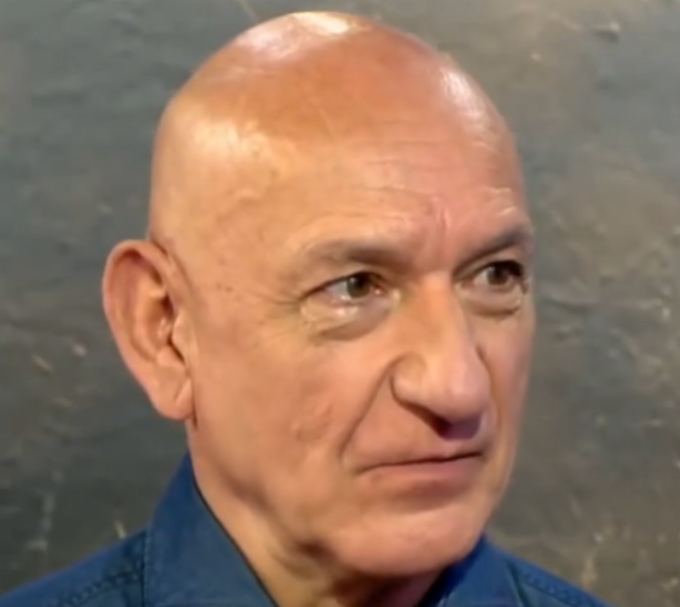
\includegraphics[width=.8\linewidth]{figures/method1}
		\caption{FaceForensics++}\label{fig:sub1}
	\end{subfigure}%
	\hspace{-5mm}
	\begin{subfigure}{.45\textwidth}
		\centering
		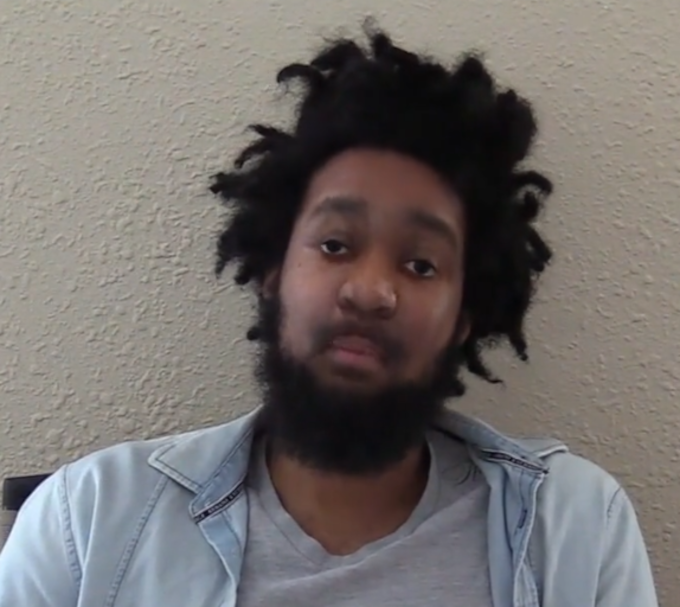
\includegraphics[width=.8\linewidth]{figures/method2}
		\caption{DFDC}\label{fig:sub2}
	\end{subfigure}
	\vspace{5mm} % Adjust the vertical spacing if needed
	\begin{subfigure}{.45\textwidth}
		\centering
		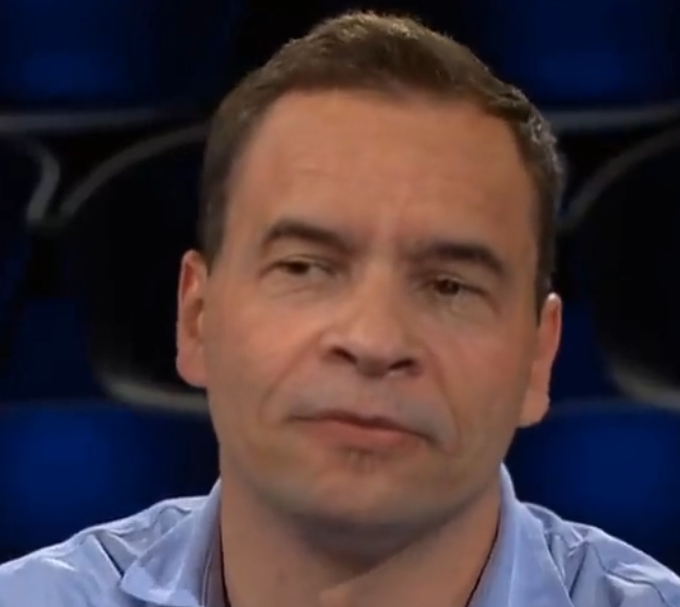
\includegraphics[width=.8\linewidth]{figures/method3}
		\caption{FFIW}\label{fig:sub3}
	\end{subfigure}%
	\hspace{-5mm}
	\begin{subfigure}{.45\textwidth}
		\centering
		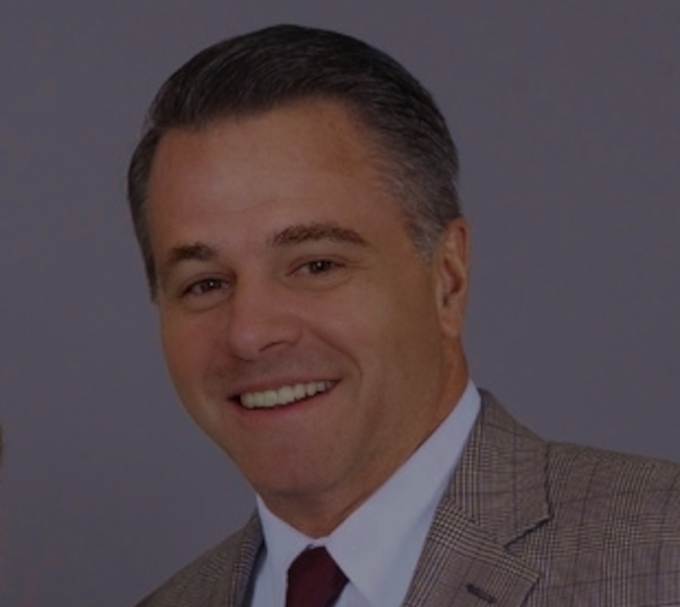
\includegraphics[width=.8\linewidth]{figures/method4}
		\caption{OpenForensics}\label{fig:sub4}
	\end{subfigure}
	\caption{Sample deepfake images taken from FaceForensics++~\cite{roessler2019faceforensicspp},
		DFDC~\cite{dolhansky2020deepfake}, FFIW~\cite{Zhou_2021_CVPR}
		and OpenForensics~\cite{ltnghia-ICCV2021}.}\label{fig:sample-deepfakes}
\end{figure}
